\documentclass[10pt, final]{article}
% \documentclass[10pt,technote]{IEEEtran}
\usepackage[a4paper,width=185mm,top=20mm,bottom=20mm]{geometry}
\usepackage{pythonhighlight}
\usepackage{url}
\usepackage{lipsum}
\usepackage{amsmath}
\usepackage{multicol}
\setlength{\columnsep}{1cm}
\usepackage{graphicx}
\graphicspath{{../results/}{../immagini/}}
\DeclareGraphicsExtensions{.png}
\usepackage{wrapfig}
\usepackage[font=small,labelfont=bf]{caption}
\usepackage{setspace}
\usepackage{caption}
\usepackage{subcaption}
\usepackage{wrapfig}
\usepackage{float}
\usepackage{xcolor}
\usepackage[tikz]{mdframed}
\usepackage{colortbl}
\usepackage{MnSymbol}
\usepackage[utf8]{inputenc}
\usepackage[T1]{fontenc}
\usepackage{ascii}
\usepackage{listings}

\lstset{prebreak=\raisebox{0ex}[0ex][0ex]
        {\ensuremath{\rhookswarrow}}}
\lstset{postbreak=\raisebox{0ex}[0ex][0ex]
        {\ensuremath{\rcurvearrowse\space}}}
\lstset{breaklines=true, breakatwhitespace=true}
\lstset{numbers=left, numberstyle=\scriptsize}

\UseRawInputEncoding %%%%%%%%%%%%%%%%%%%%%%%%%OCCHIOOOOOO
\definecolor{forestgreen}{rgb}{0.0, 0.27, 0.13}
%%
%% Julia definition (c) 2014 Jubobs
%%
\lstdefinelanguage{Julia}%
  {morekeywords={abstract,break,case,catch,const,continue,do,else,elseif,%
      end,export,false,for,function,immutable,import,importall,if,in,%
      macro,module,otherwise,quote,return,switch,true,try,type,typealias,%
      using,while},%
   sensitive=true,%
   alsoother={\$},%
   morecomment=[l]\#,%
   morecomment=[n]{\#=}{=\#},%
   morestring=[s]{"}{"},%
   morestring=[m]{'}{'},%
}[keywords,comments,strings]%

\lstset{%
    language         = Julia,
    basicstyle       = \ttfamily,
    keywordstyle     = \bfseries\color{blue},
    stringstyle      = \color{magenta},
    commentstyle     = \color{forestgreen},
    showstringspaces = false,
}


\definecolor{airforceblue}{rgb}{0.36, 0.54, 0.66}
\mdfsetup{
middlelinecolor=airforceblue,%
middlelinewidth=0.2pt,%
roundcorner=5pt}
\setlength{\abovedisplayskip}{3pt}
\setlength{\belowdisplayskip}{3pt}

\renewcommand{\baselinestretch}{1}

\title{\textsc{Report 2 - Grangier-Roger-Aspect experiment analysis}}
\author{Francesco Lorenzi,      October 2020}
\date{}
\begin{document}z
\maketitle
\vspace{-25pt}

\begin{center}
	\rule[0pt]{400pt}{0.5pt}
\end{center}
\vspace{-15pt}

\begin{multicols}{2}
\subsubsection*{Summary}
The purpose of this report is to conduct a statistical analysis on a dataset collected from an experimental setup based on Grangier-Roger-Aspect experiment \cite{grangier}. 

In a second part, an application of photon arrival statistics is also showed: using a dataset from coherent light photon detection random data is generated and used to approximate the base of the natural logarithm $e$.

\section{Photon indivisibility experiment}
The experiment developed by Grangier, Roger and Aspect in 1986 consist in verify by statistical means on photomultipliers hits, that a single  photon, after impinging on a beam splitter, is present in only one of the beams after, and so it is indivisible. 
From the theoretical point of view, this experiment confirms the quanized nature of radiation, as the classical model for photodetection, which predicts correlation between detection along the two branches, is completely contradicted by the data.
\subsection*{Experimental setup}
Even if the description of the experiment is straightfoward, an additional technique is needed to prevent detector noise from making the data unintelligible.
So a source which emits photon \emph{in couples} is used, one is sent to a separate detector, whereas the other is sent to the setup described before. In that way the first photon triggers a \emph{gate} signal that allow count from the other detector to be validated.

Altought in the original experiment this feature was hardwired with electronics, in our setup all events are collected regardless, and the \emph{gate} signal is be applied separately in post-processing.
\begin{mdframed}
    \begin{figure}[H]
        \begin{subfigure}{\textwidth}
            \centering
            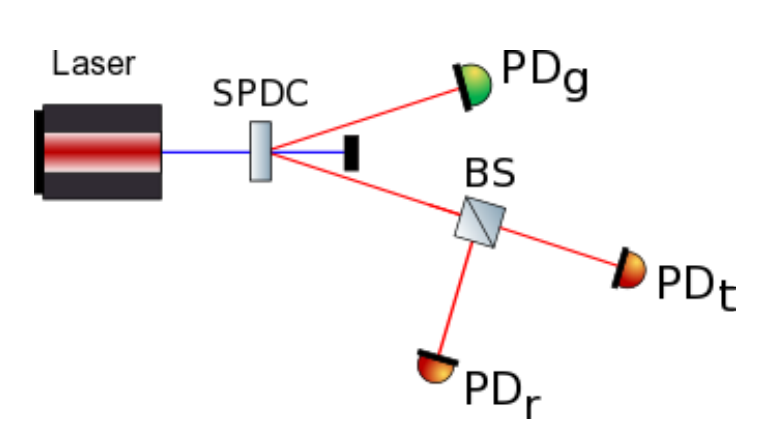
\includegraphics[width = 0.9\textwidth]{../images/our_setup.png}
            \caption{Actual setup}
            \label{our}
        \end{subfigure}

        \begin{subfigure}{\textwidth}
            \centering
            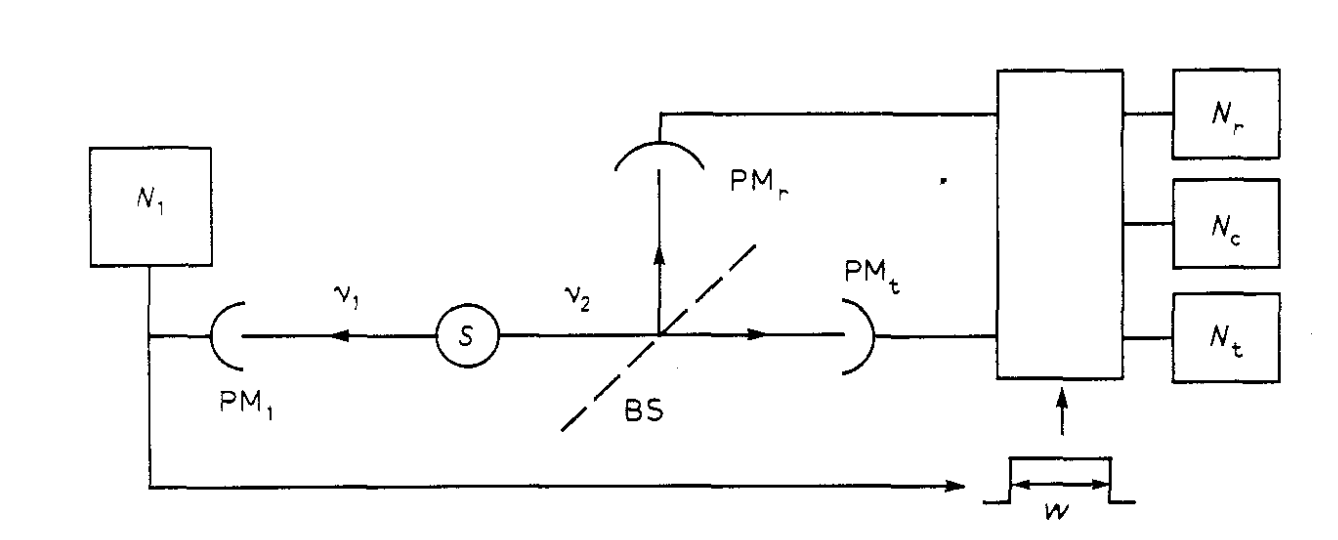
\includegraphics[width = \textwidth]{../images/original.png}
            \caption{Original setup}
        \end{subfigure}
        \caption{Experimental setup scheme}
    \end{figure}
\end{mdframed}
In the setup in \ref{our} all the pulses from the detectors $PM_*$ are collected by a time-tagger on a common time scale in three different channels.

The goal of the experiment is to verify that 
\begin{equation}
    \alpha = 
\end{equation}
is less than asdvaonvaoirnvao predicted by classical theory

\subsection*{Analysis}
As anticipated, before counting double and triple coincidences, a preprocessing step is necessary. First of all, we reject events on the same channel which are distanced by less than $3900$ machine time units defined by $1 MTU = 80.955 ps$. In fact, events whose difference in time is less than $\approx 0.315 \mu s$ could be \emph{afterpulses}, artifacts of the detection electronics.

In a second step, we must filter the data with a suitable \emph{gate} function, triggered by the events on 

In order to build a correct gate function, .

The difference between events caused by two photons belonging to the same pair, respectively on the gate detector and on one of the transmitted or reflected detectors, must be less that a given constant time. This can be said for physical reasons: (NEGLECTING RELATIVISTIC CONSIDERATIONS???) the pulses reach the time-tagger front end after the propagation of each photon along the optical bench, and the signal along the RG cable. The maximum time delay must be in the order of $\sim 10 ns$, so we filter only events around $\pm 100 MTU$ away from the nearest gate event.
\subsection*{Interpretation of results}

\section{Random Number Generation}


\section*{Conclusions}

\bibliography{References}
\begin{thebibliography}{99}
  \bibitem{grangier} Grangier, Roger, Aspect
\end{thebibliography}
\end{multicols}




\hrulefill
\subsection*{Code}

\renewcommand{\baselinestretch}{0.5}
\begin{mdframed}
  \begin{lstlisting}
    module Analyzer
using Plots
using Printf
import Plotly
import PGFPlots
import Statistics
import ProgressMeter

export delay_estimator, main, loader, difference_info, gated_counter, single_chan_stat

Plots.gr()
default(show = true)
# PyPlot.clf()
# println(PyPlot.backend)
const machine_time = 80.955e-12

function loader(;aft_filter = true)
    println("Loading...")
    s = "./tags.txt"
    a = readlines(s)
    for y in a
        filter(x -> !isspace(x), y)
    end
    i=0
    b = Array{Int, 2}(undef, 2, length(a))

    b[1, :] = [parse(Int, split(x, ";")[1]) for x in a]
    b[2, :] = [parse(Int, split(x, ";")[2]) for x in a]


    tags = Array{Int, 2}(undef, 3, length(b))
    fill!(tags, 0)
    println(typeof(tags))
    k = Array{Int, 1}(undef, 3) # k[i] will be the total count of trigger events on channel i
    fill!(k, 1)
    i=0
    cnt = 0
    aft = Array{Int, 1}(undef, 3)
    fill!(aft, 0)
    if (aft_filter)
        aft_const = 3900
    else
        aft_const = 0
    end
    for i = 1:length(a)
         if (i<8 || tags[ b[2, i]-1, k[b[2, i]-1] - 1 ] + aft_const < b[1, i] )
            tags[ b[2, i]-1, k[b[2, i]-1] ] = b[1, i]
            k[b[2, i] - 1] += 1
        else
            # println("Afterpulse on CH-", b[2, i] - 1)
            aft[b[2, i] - 1] +=1
        end
    end

    println("Number of valid hits")
    @printf("\t n. of transmitted hits   : %6d \n", k[1])
    @printf("\t n. of reflected hits     : %6d \n", k[2])
    @printf("\t n. of gate hits          : %6d \n", k[3])
    println("T+R = ", k[1]+k[2], ", G = ", k[3])
    println("Number of afterpulses:")
    @printf("\t chan 1 - transmitted (2) : %6d \n", aft[1])
    @printf("\t chan 2 - reflected (3)   : %6d \n", aft[2])
    @printf("\t chan 3 - gate (4)        : %6d \n", aft[3])
    println("Percentage of afterpulses")
    @printf("\t chan 1 - transmitted (2) : %4.1f %% \n", aft[1]/k[1] * 100)
    @printf("\t chan 2 - reflected (3)   : %4.1f %% \n", aft[2]/k[2] * 100)
    @printf("\t chan 3 - gate (4)        : %4.1f %% \n", aft[3]/k[3] * 100)
    return (tags, k);
end

function delay_estimator((tags, k); mode = "gate_first")
    println("Analyzing...")
    machine_time = 80.955e-12
    diff1 = Array{Int, 1}(undef, k[1])
    diff2 = Array{Int, 1}(undef, k[2])
    fill!(diff1, 0)
    fill!(diff2, 0)
    if mode == "gate_last"
        g1 = -1         # BE CAREFUL : NOT A REAL GATE EVENT
        g2 = tags[3, 1]
        n = 1
        # Retarded gate method - positive diff
        for i = 2:k[3]
            while (tags[1, n]<g2 && n<k[1])
                diff1[n] = g2 - tags[1, n]
                n += 1
            end
            g2 = tags[3, i]
        end

        g1 = -1         # BE CAREFUL : NOT A REAL GATE EVENT
        g2 = tags[3, 1]
        n = 1
        for i = 2:k[3]
            while (tags[2, n]<g2 && n<k[2])
                diff2[n] = g2 - tags[2, n]
                n += 1
            end
            g2 = tags[3, i]
        end
    elseif mode == "gate_first"
        # Anticipated gate method - positive diff
        g1 = -1         # BE CAREFUL : NOT A REAL GATE EVENT
        g2 = tags[3, 1]
        n = 8
        for i = 2:k[3]
            while (tags[1, n]<g2 && n<k[1])
                diff1[n] = tags[1, n] - g1
                n += 1
            end
            g1 = g2
            g2 = tags[3, i]
        end
        diff1 = diff1[8:length(diff1)]

        g1 = -1         # BE CAREFUL : NOT A REAL GATE EVENT
        g2 = tags[3, 1]
        n = 8
        for i = 2:k[3]
            while (tags[2, n]<g2 && n<k[1])
                diff2[n] = tags[2, n] - g1
                n += 1
            end
            g1 = g2
            g2 = tags[3, i]
        end
        diff2 = diff2[8:length(diff2)]
    else
        # Minimum distance method
        g1 = -100000000         # BE CAREFUL : NOT A REAL GATE EVENT
        g2 = tags[3, 1]
        n = 1
        for i = 2:k[3]
            while (tags[1, n]<g2 && n<k[1])
                if ((tags[1, n] - g1) <  (g2 - tags[1, n]))
                    diff1[n] = tags[1, n] - g1
                else
                    diff1[n] = tags[1, n] - g2
                end
                n += 1
            end
            g1 = g2
            g2 = tags[3, i]
        end
        g1 = -100000000         # BE CAREFUL : NOT A REAL GATE EVENT
        g2 = tags[3, 1]
        n = 1
        for i = 2:k[3]
            while (tags[2, n]<g2 && n<k[1])
                if ((tags[2, n] - g1) <  (g2 - tags[2, n]))
                    diff2[n] = tags[2, n] - g1
                else
                    diff2[n] = tags[2, n] - g2
                end
                n += 1
            end
            g1 = g2
            g2 = tags[3, i]
        end
    end

    # max_delay = 7.5 # [ns]
    # max_clicks = max_delay * 1e-9/machine_time
    max_clicks = 80
    max_delay = max_clicks * machine_time / 1e-9
    @printf("PRE-filtering at max delay = %d ns \n ", max_delay)
    # unreal difference filter
    filter!(x-> (x< max_clicks), diff1)
    filter!(x-> (x< max_clicks), diff2)

    filter!(x -> (x>0), diff2)

    difference_info(diff1, diff2, k)
    μ1 = Statistics.mean(diff1)
    μ2 = Statistics.mean(diff2)
    σ1 = sqrt(Statistics.var(diff1 .- μ1))
    σ2 = sqrt(Statistics.var(diff2 .- μ2)) 

    return [μ1, σ1, μ2, σ2]
end

function single_chan_stat((tags, k); chan = 3)
    machine_time = 80.955e-12
    series = tags[chan, :]
    diff = Array{Int, 1}(undef, length(series)-1)
    for i = 1:length(series)-1
        diff[i] = series[i+1] - series[i]
    end
    filter!(z -> (z>0), diff)
    max_diff = maximum(diff)
    println("min: ", minimum(diff))
    bin_num = 1000

    bin_step =Int(ceil(max_diff / bin_num))+1
    println("max diff : ", max_diff, " bin step", bin_step)
    hist = Array{Int, 1}(undef, bin_num)
    fill!(hist, 0)
    i = 1
    for i = 1:length(diff)
        hist[Int(floor((diff[i]) / bin_step)) + 1] += 1
    end
    @printf("minimum difference between gate event: %10d clicks -> %5.2f ns \n",minimum(diff) , minimum(diff)*machine_time/1e-9
    )

    prob = hist / sum(hist)
    accum = 0
    i = 1
    for i = 1:bin_num
        accum += (i-1) * prob[i]
    end
    mu = accum
    var = 0
    sk_acc = 0
    kr_acc = 0 
    for i = 1:bin_num
        var += (i-1 - mu)^2 * prob[i]
        sk_acc += (i-1 - mu)^3 * prob[i]
        kr_acc += (i-1 - mu)^4 * prob[i]
    end
    sigma = sqrt(var)
    sk = sk_acc 
    kr = kr_acc 
    theo_mom = poisson_moments(mu)
    @printf("Statistical analysis of gate events process:\n")
    @printf("\t δ mean                : %5.3f \n", mu  - theo_mom[1])
    @printf("\t δ variance            : %5.3f \n", var - theo_mom[2])
    @printf("\t δ skewness non std    : %5.3f \n", sk  - theo_mom[3])
    @printf("\t δ kurtosis non std    : %5.3f \n", kr  - theo_mom[4])

    fig = Plots.plot((1:bin_num)*bin_step,
                         [log10(h) for h in hist],
                         show=true,
                         xlabel = "absolute difference between gate events (clicks)",
                         size = (1200, 800))
    savefig(fig, string("./images/", chan, "-single_chan.pdf"))
end

function poisson_moments(mu)
    return [mu, mu, 1/sqrt(mu), 1/mu]
end

function bose_ein_moments(mu)
    sigma = sqrt(mu + mu^2)
    return [mu,
            sigma^2,
            (mu + 3*mu^2 + 2*mu^3)/sigma^3,
            (mu + 10*mu^2 + 18*mu^3 + 9*mu^4)/sigma^4]
end

function difference_info(diff1, diff2, k)
    machine_time = 80.955e-12
    println("Difference Info...")
    max_diff1 = maximum(diff1)
    min_diff1 = minimum(diff1)
    max_diff2 = maximum(diff2)
    min_diff2 = minimum(diff2)
    @printf("1) maximum difference      : %10d \n", max_diff1)
    @printf("1) minimum difference      : %10d \n", min_diff1)
    @printf("1) maximum time difference  (ns)  : %10.4f \n", max_diff1 * machine_time * 1e9)
    @printf("1) minimum time difference  (ns)  : %10.4f \n", min_diff1 *machine_time * 1e9)

    @printf("2) maximum difference      : %10d \n", max_diff2)
    @printf("2) minimum difference      : %10d \n", min_diff2)
    @printf("2) maximum time difference  (ns)  : %10.4f \n", max_diff2*machine_time * 1e9)
    @printf("2) minimum time difference  (ns)  : %10.4f \n\n", min_diff2*machine_time * 1e9)

    @printf("1) Fraction of accepted hits : %d / %d = %4.2f \n", length(diff1), k[1], length(diff1)/k[1])
    @printf("2) Fraction of accepted hits : %d / %d = %4.2f\n", length(diff2), k[2], length(diff2)/k[2])

    # Want to show exactly 100 bins in histogram
    mod = Int(ceil(maximum([length(diff1), length(diff2)]) / 1e4)) # TO BE MODIFIED

    # plot clicks 
    x_delays1 = (min_diff1:mod:max_diff1)
    x_delays2 = (min_diff2:mod:max_diff2)

    bin_num1 = Int(floor((max_diff1-min_diff1) / mod)) + 1
    println("bins 1: ", bin_num1)
    bias1 = Int(floor(-min_diff1/mod))
    hist1 = Array{Int, 1}(undef, bin_num1)
    fill!(hist1, 0)
    i = 1
    while (i<=length(diff1))
        hist1[Int(floor((diff1[i] - min_diff1) / mod))+1] += 1
        i += 1
    end

    bin_num2 = Int(floor((max_diff2-min_diff2) / mod)) + 1
    bias2 = Int(floor(-min_diff2/mod))
    println("bins 2: ", bin_num2)
    hist2 = Array{Int, 1}(undef, bin_num2)
    fill!(hist2, 0)
    i = 1
    while (i<=length(diff2))
        hist2[Int(floor((diff2[i] - min_diff2) / mod))+1] += 1
        i += 1
    end
    μ1 = Statistics.mean(diff1)
    μ2 = Statistics.mean(diff2)
    σ1 = sqrt(Statistics.var(diff1 .- μ1))
    σ2 = sqrt(Statistics.var(diff2 .- μ2)) 

    if (length(hist1)<600 && length(hist2)<600)
        println("Plotting...")
        # fig = Plotly.figure()
        n_σ = 2
        fig = Plots.bar(x_delays1,
                         hist1,
                         show=true,
                         title = string("Event delay and ±", n_σ, "σ decision region"),
                         xlabel = "absolute difference from gate event (clicks)",
                         ylabel = "Frequency", 
                         label = "transmitted photon delay", 
                         size = (1000, 600))
        Plots.bar!(x_delays2, hist2, label = "reflected photon delay")
        rectangle(w, h, x, y) = Plots.Shape(x .+ [0,w,w,0], y .+ [0,0,h,h])

        recr = rectangle(2*n_σ*σ1, maximum([maximum(hist1), maximum(hist2)]), μ1-n_σ*σ1, 0)
        rect = rectangle(2*n_σ*σ2, maximum([maximum(hist1), maximum(hist2)]), μ2-n_σ*σ2, 0)
        Plots.plot!(recr, linewidth = 2, opacity = 0.1, color=:blue, label="transmitted decision region")
        Plots.plot!(rect, linewidth = 2, opacity = 0.1, color=:red, label="reflected decision region")

        display(fig)
        savefig("./images/delays.pdf")
    else
        println("Too long to plot...")
    end
end

# need to decide what method to use -> we use  GATE -> REFLECTED -> TRANSMITTED
function gated_counter((tags, k), params; mode = "full-width")
    println("Gated counting...")
    μ1 = params[1]
    σ1 = params[2]
    μ2 = params[3]
    σ2 = params[4]

    @printf("mean reflected   : %6.4f \n", params[1])
    @printf("stdd reflected   : %6.4f \n", params[2])
    @printf("mean tramsmitted : %6.4f \n", params[3])
    @printf("stdd tramsmitted : %6.4f \n", params[4])
    N_1 = length(tags[3, :])
    intervals = [6]
    # Gate function (not counting with multiple hits)
    for n_σ in intervals
        x = 1
        r_hit = false
        refl = 0
        multiple_refl = 0
        y = 1
        t_hit = false
        tran = 0
        multiple_tran = 0
        coincidences = 0
        if (mode == "confidence") 
            for i=1:length(tags[3, :])-1
                r_hit = false
                t_hit = false  
                while  tags[1, x] < -n_σ*σ1 + tags[3, i] + μ1
                    x += 1
                end
                while -n_σ*σ1 + tags[3, i] + μ1 <= tags[1, x] < +n_σ*σ1 + tags[3, i] + μ1 && tags[1, x] < tags[3, i+1] 
                    r_hit = true
                    x += 1
                end
                if r_hit
                    refl += 1
                end

                while  tags[2, y] < -n_σ*σ2 + tags[3, i] + μ2 
                    y += 1
                end
                while -n_σ*σ2 + tags[3, i] + μ2 <= tags[2, y] < +n_σ*σ2 + tags[3, i] + μ2  && tags[2, y] < tags[3, i+1]
                    t_hit = true
                    y += 1
                end
                if t_hit
                    tran += 1
                end
                if r_hit && t_hit
                    coincidences += 1
                end
            end
        else
            for i=1:length(tags[3, :])-1
                r_hit = false
                t_hit = false 
                while tags[1, x] < tags[3, i]
                    x += 1
                end
                while tags[3, i] < tags[1, x] <= tags[3, i+1] 
                    r_hit = true
                    x += 1
                end
                if r_hit
                    refl += 1
                end

                while tags[2, y] < tags[3, i]
                    y += 1
                end
                while tags[3, i] < tags[2, y] <= tags[3, i+1]
                    t_hit = true
                    y += 1
                end
                if t_hit
                    tran += 1
                end
                if r_hit && t_hit
                    coincidences += 1
                end
            end
        end
        @printf("Measurement with ciao confidence \n")
        prob_refl = refl / N_1
        prob_tran = tran / N_1
        prob_triple = coincidences / N_1
        α = prob_triple/ (prob_refl * prob_tran)
        @printf("\t gate         hits :  %9d \n", N_1)
        @printf("\t reflected    hits :  %9d \n", refl)
        @printf("\t transmitted  hits :  %9d \n", tran)
        @printf("\t coincidences hits :  %9d \n", coincidences)
        @printf(" ----------------------\n")
        @printf("\t P[double]         : %9.8f \n", prob_refl + prob_tran)
        @printf("\t P[triple]         : %9.8f \n", prob_triple)
        @printf("\t Alpha             : %9.8f \n", α)
    end
end

function main()
    println("Nothing to do...")
end
end
  \end{lstlisting}
\end{mdframed}

\end{document}